\documentclass[12pt]{article}
\usepackage{setspace,graphicx,amsmath,geometry,fontspec,titlesec,soul,bm,subfigure,alphalph,enumitem}
\titleformat{\section}[block]{\LARGE\bfseries}{\arabic{section}}{1em}{}[]
\titleformat{\subsection}[block]{\Large\bfseries\mdseries}{\arabic{section}.\arabic{subsection}}{1em}{}[]
\titleformat{\subsubsection}[block]{\normalsize\bfseries}{\arabic{subsection}-\alph{subsubsection}}{1em}{}[]
\titleformat{\paragraph}[block]{\small\bfseries}{[\arabic{paragraph}]}{1em}{}[]
\setmainfont{Times New Roman}
\renewcommand{\baselinestretch}{1.15}
\renewcommand\contentsname{Inhaltverzeichnis}
\geometry{a4paper,left=2.5cm,right=2.5cm,top=2.5cm,bottom=2.5cm}
\usepackage{alphalph}
\renewcommand*{\thesubfigure}{%
	\alphalph{\value{subfigure}}%
}%
\begin{document}
	\newpagestyle{main}{            
		\sethead{Ziqing Yu}{Physikalische Geodäsie Übung 6}{3218051}     
		\setfoot{}{\thepage}{}     
		\headrule                                     
		\footrule                                       
	}
	\pagestyle{main}
\tableofcontents
\newpage
\section{Task 1}
\subsection{Rodrigues-Ferrers}
Mit Rodrigues-Ferrers Verfahren kann man so rechnen:
\begin{equation*}
\bar{P}_{l,m}(t)\begin{cases}
\sqrt{2l+1}P_{l,m}(t) \quad &m=0 \\
\sqrt{2(2l+1)\frac{(l-m)!}{(l+m)!}} P_{l,m}(t) \quad &m>0
\end{cases}
\end{equation*}
\begin{figure*}[ht]\centering
	\subfigure[Legendre Funktion]{
		\includegraphics[width=0.65\textwidth]{pl10ro.png}}
	\subfigure[Spherical Harmonics]{
		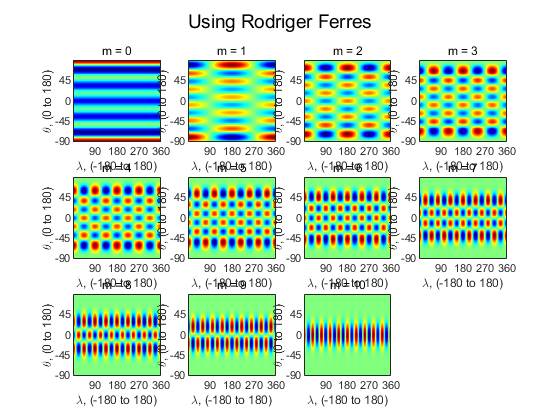
\includegraphics[width=0.65\textwidth]{Yl10ro.png}}
\end{figure*}
\newline
Es ist deutlich zu sehen, die Nulldurchgänge gleich $l - m$ in erste Bild. Die Nulldurchgänge sind gleich $l - m$ in Nord-Süd Richtung und gleich $2m$ in Ost-West\newpage
\subsection{Rekursiv}
Die Formeln von Rekursive Verfahren stellen darunter:
\begin{align*}
Initial: & \bar{P}_{0,0}(t) = 1\quad \bar{P}_{1,0}(t) = \sqrt{3}t\quad \bar{P}_{1,1}(t) = \sqrt{3(1-t^2)}\\
Sectorial: & \bar{P}_{l,l}(t) = \sqrt{\frac{2l+1}{2l}} \sqrt{1-t^2}\bar{P}_{l-1,l-1}(t) \\
Othre: & \bar{P}_{l,m}(t) = \sqrt{\frac{2l+1}{(l+m)(l-m)}} \{\sqrt{2l-1} t \bar{P}_{l-1,m}(t) - \sqrt{\frac{(l-1+m)(l-1-m)}{2l-3}} \bar{P}_{l-1,m}(t)\}
\end{align*}
\begin{figure*}[ht]\centering
	\subfigure[Legendre Funktion]{
		\includegraphics[width=0.65\textwidth]{pl10rec.png}}
	\subfigure[Spherical Harmonics]{
		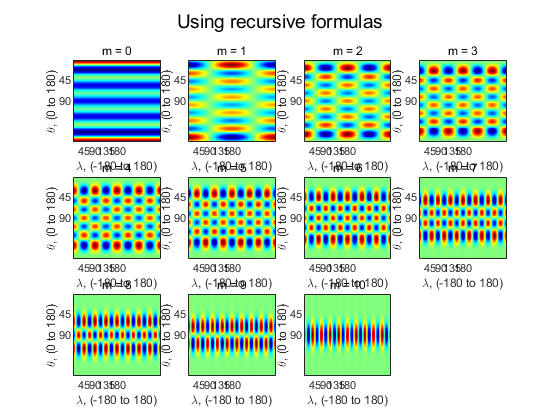
\includegraphics[width=0.65\textwidth]{Yl10rec.png}}
\end{figure*}
\newline
Die Ergebnisse sind gleich wie mit Rodrigues-Ferrers Verfahren \newpage
\section{Task 2}
Theoretisch gibt es eine Gleichung:
\begin{equation*}
P_l(\cos \Phi_{PQ}) = \frac{1}{2l+1} \sum_{m=0}^{l} P_{lm}(\cos \theta_P) P_{lm}(\cos(\theta_Q))\{\cos m \lambda_P \cos m \lambda_Q + \sin m \lambda_P \sin m \lambda_Q\}
\end{equation*}
Für $P$ und $Q$ mit gleichen Länge:
\begin{equation*}
P_l(\cos \Phi_{PQ}) = \frac{1}{2l+1} \sum_{m=0}^{1} \bar{P}_{lm}(\cos \theta_P) \bar{P}_{lm}(\cos \theta_Q)
\end{equation*}
Für $\theta_P = 90°$ und $\theta_Q = [0° 90°]$ können wir linke Seite und Rechte Seite vergleichen. Linke Seite rechnen wir mit dem Verfahren von Rodriger-Ferrers, rechte Seite rechnen wir mit dem rekursivem Verfahren. Die Unterschiede von $l = 0 $ bis $100$ \newline
\begin{figure*}[ht]\centering
	\subfigure[l = 0 bis 8]{
		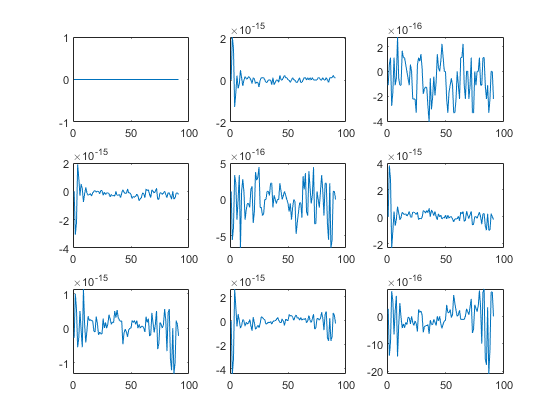
\includegraphics[width=0.45\textwidth]{task2_1.png}}
	\subfigure[l = 9 bis 17]{
		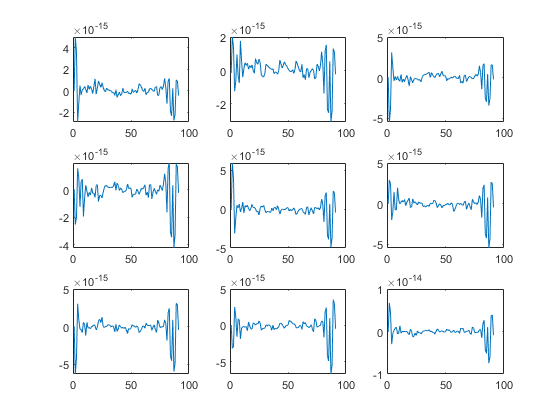
\includegraphics[width=0.45\textwidth]{task2_2.png}}
	\subfigure[l = 18 bis 26]{
		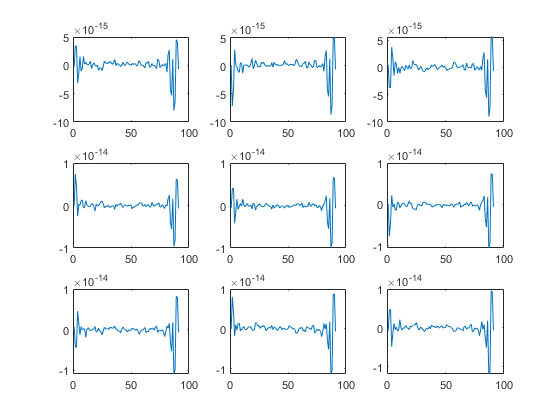
\includegraphics[width=0.45\textwidth]{task2_3.png}}
	\subfigure[l = 27 bis 35]{
		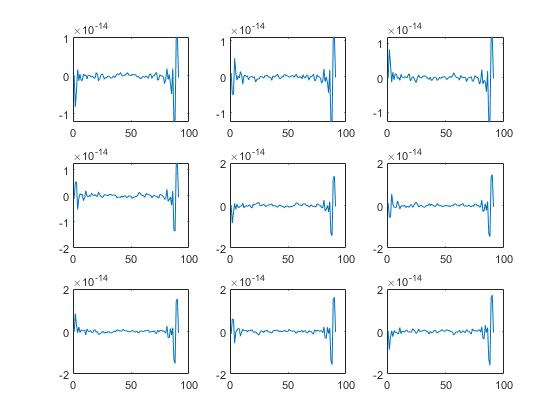
\includegraphics[width=0.45\textwidth]{task2_4.png}}	
\end{figure*}
\begin{figure*}[ht]\centering
	\subfigure[l = 36 bis 44]{
	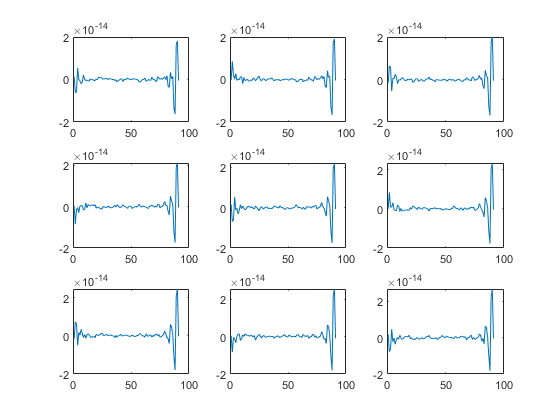
\includegraphics[width=0.3\textwidth]{task2_5.png}}	
\subfigure[l = 45 bis 53]{
	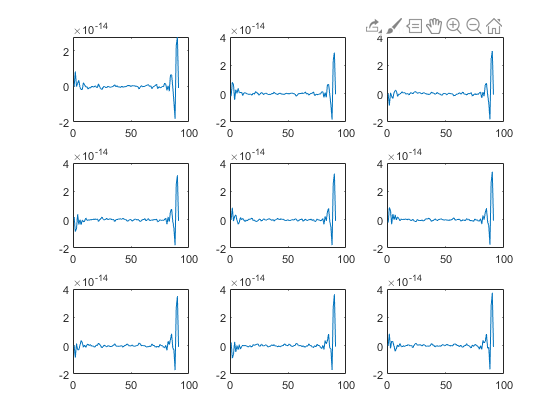
\includegraphics[width=0.3\textwidth]{task2_6.png}}
\subfigure[l = 54 bis 62]{
	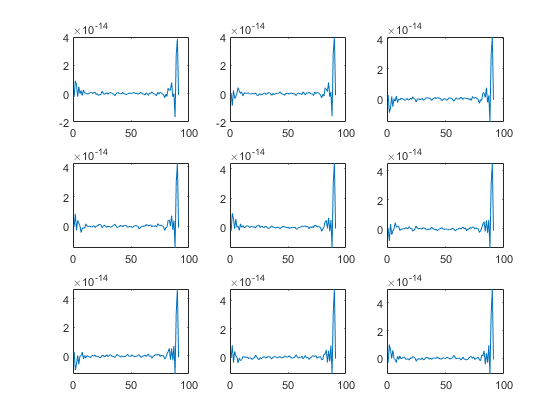
\includegraphics[width=0.3\textwidth]{task2_7.png}}
\subfigure[l = 63 bis 71]{
	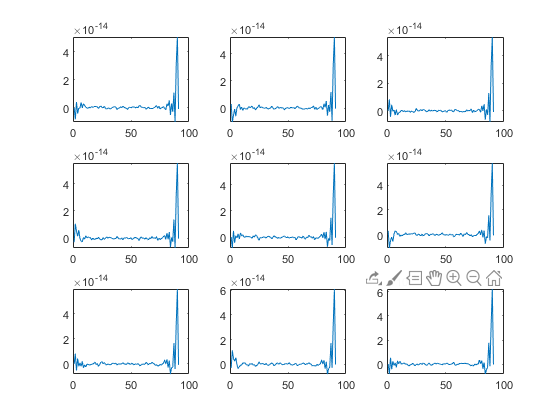
\includegraphics[width=0.3\textwidth]{task2_8.png}}
\subfigure[l = 72 bis 80]{
	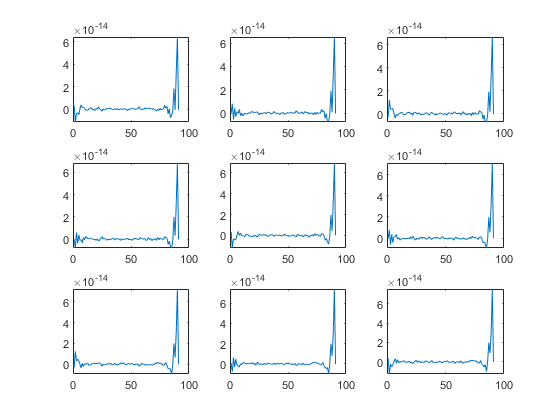
\includegraphics[width=0.3\textwidth]{task2_9.png}}
\subfigure[l = 81 bis 89]{
	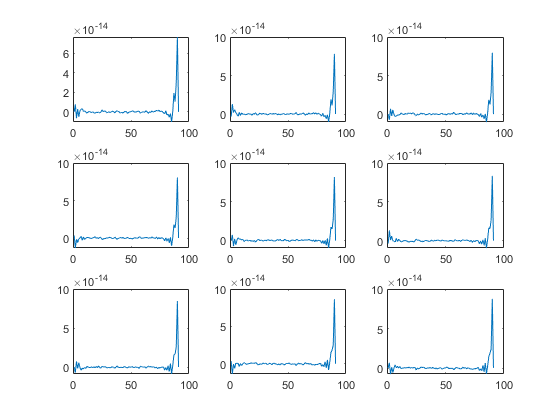
\includegraphics[width=0.3\textwidth]{task2_10.png}}	
\subfigure[l = 90 bis 98]{
	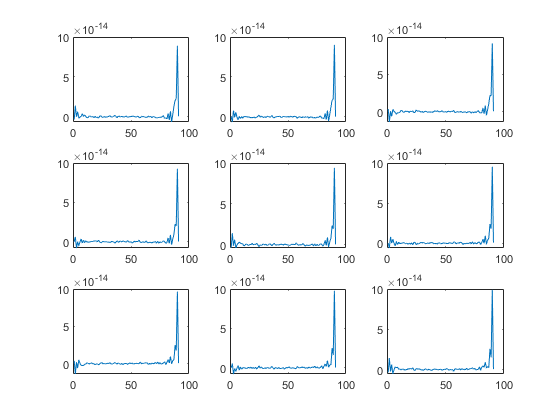
\includegraphics[width=0.3\textwidth]{task2_11.png}}	
\subfigure[l = 99 bis 101]{
	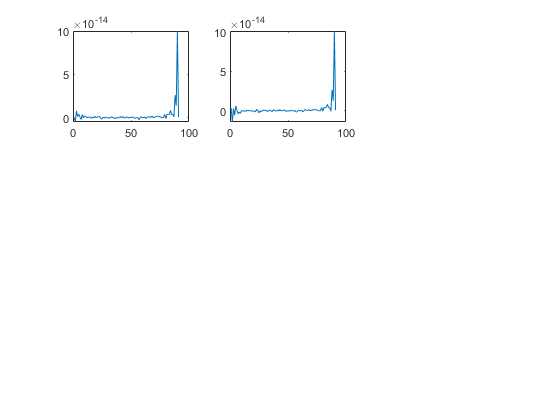
\includegraphics[width=0.3\textwidth]{task2_12.png}}
\end{figure*}
\noindent Die Unterschied erhöht sich mit größere Grad $l$, obwohl die Unterschied zwischen beiden Seite sehr klein sind.\newpage 
\section{task 3}
Wenn $\theta_P = \theta_Q = [0° 180°]$, sind $P_l(1) = 1 = \frac{1}{2l+1}\sum_{m=0}^{l}\bar{P}_{lm}^2(\cos \theta)$, mit gleichem Verfahren wie in task 2 können wir finden, dass für alle Grad $\frac{1}{2l+1}\sum_{m=0}^{l}\bar{P}_{lm}^2(\cos \theta) = 1$ sind.  
\begin{figure*}[ht]\centering
	\subfigure[l = 0 bis 8]{
		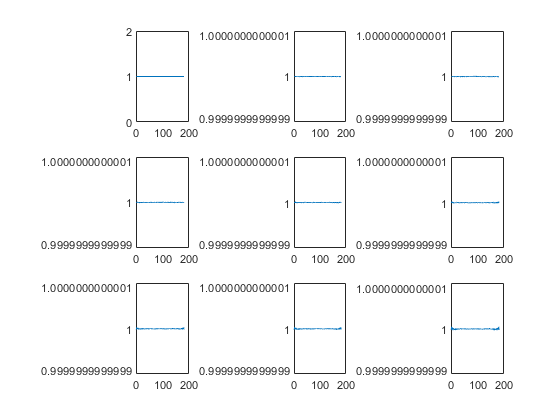
\includegraphics[width=0.35\textwidth]{t3_1.png}}
	\subfigure[l = 9 bis 17]{
		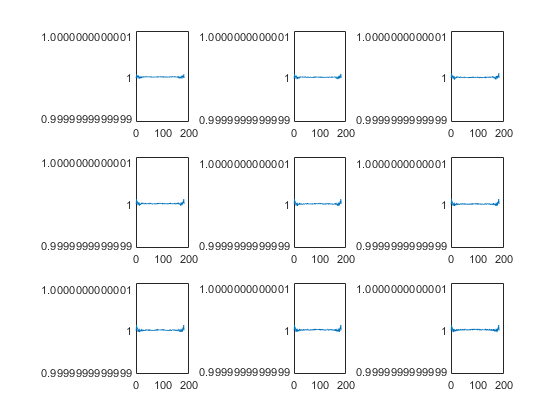
\includegraphics[width=0.35\textwidth]{t3_2.png}}
\end{figure*}
\begin{figure*}[ht]\centering
	\subfigure[l = 18 bis 26]{
	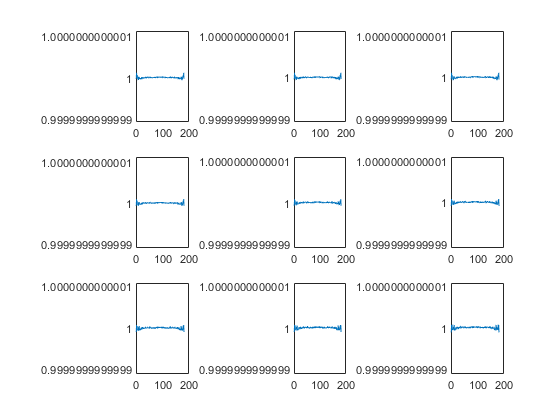
\includegraphics[width=0.3\textwidth]{t3_3.png}}
\subfigure[l = 27 bis 35]{
	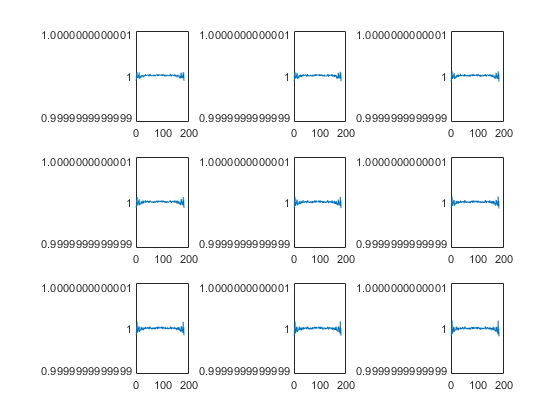
\includegraphics[width=0.3\textwidth]{t3_4.png}}	
\subfigure[l = 36 bis 44]{
	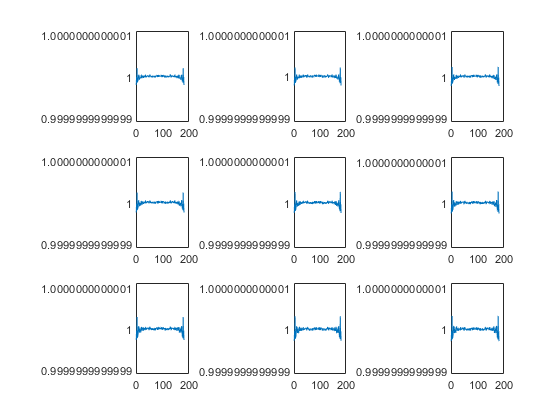
\includegraphics[width=0.3\textwidth]{t3_5.png}}	
\subfigure[l = 45 bis 53]{
	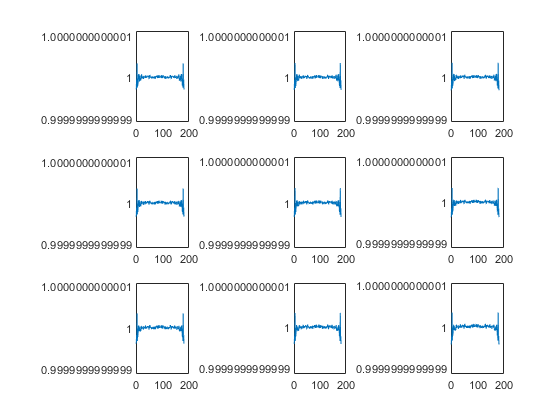
\includegraphics[width=0.3\textwidth]{t3_6.png}}
\subfigure[l = 54 bis 62]{
	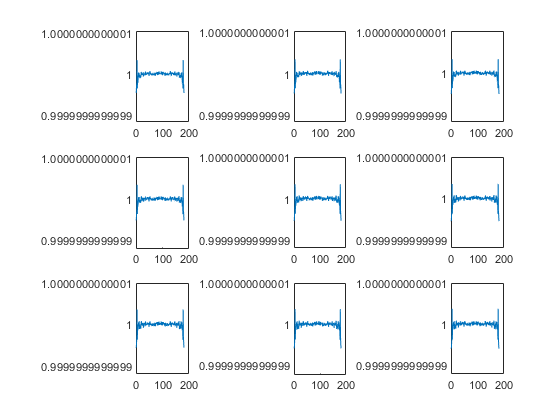
\includegraphics[width=0.3\textwidth]{t3_7.png}}
\subfigure[l = 63 bis 71]{
	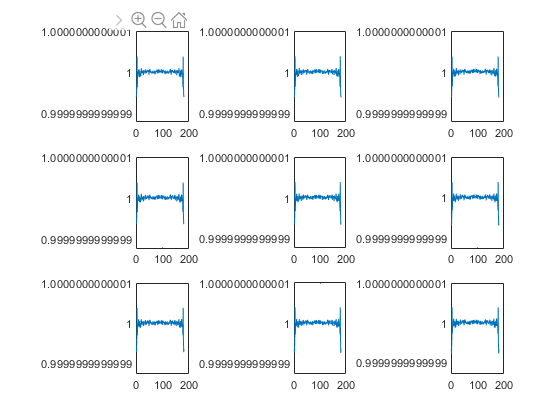
\includegraphics[width=0.3\textwidth]{t3_8.png}}
\subfigure[l = 72 bis 80]{
	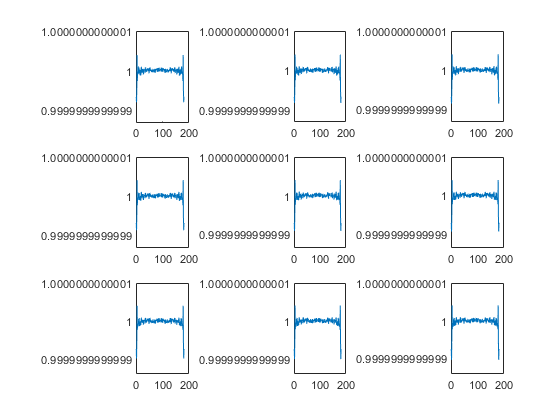
\includegraphics[width=0.3\textwidth]{t3_9.png}}
\subfigure[l = 81 bis 89]{
	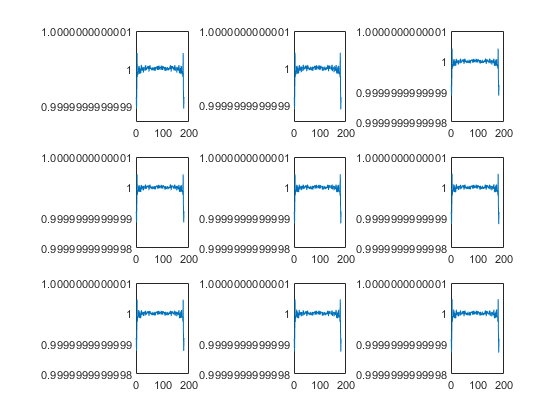
\includegraphics[width=0.3\textwidth]{t3_10.png}}	
\subfigure[l = 90 bis 98]{
	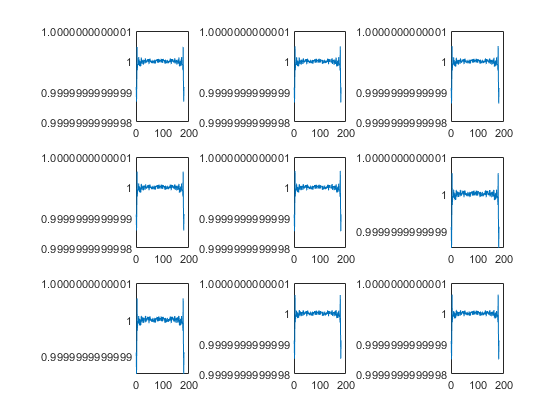
\includegraphics[width=0.3\textwidth]{t3_11.png}}	
\subfigure[l = 99 bis 101]{
	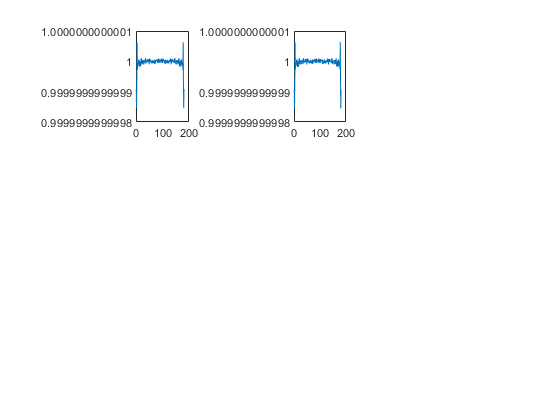
\includegraphics[width=0.3\textwidth]{t3_12.png}}
\end{figure*}
\newpage
\section{Task 4}
Die Koordinaten von P: $\lambda = 11°$, $\theta = 43°$, $r = 6379245.458$, Die Gravitation und Schwerkraft werden in dieser Aufgabe berechnet.(hier ist $l=36$)
\begin{gather*}
V(\lambda,\theta,r) = \frac{GM}{R}\sum_{l=0}^{37}(\frac{R}{r})^{l+1}\sum_{m=0}^{l}\bar{P}_{l,m}(\cos \theta)(\bar{c}_{l,m} \cos m \lambda + \bar{s}_{l,m} \sin m \lambda) = 62463927.101\\
V_c(\lambda,\theta,r) = \frac{1}{2} \omega^2 r^2 \sin^2 \theta = 50324.829\\
W = V + V_c = 62514251.930
\end{gather*}
\end{document}